\section{Introduction}
\label{sec:introduction}

\subsection{Research Background}
\label{subsec:research-background}

\hspace*{\parindent}The ubiquity of smartphones has fundamentally transformed human communication and working paradigms. Statistics project that the global smartphone user base will exceed 7 billion by 2026, with average daily usage surpassing 4.5 hours. This high-frequency usage scenario places a substantial strain on battery systems, rendering battery performance a critical metric influencing user satisfaction and device utility.

As the predominant power source, Lithium-ion batteries operate via complex mechanisms that are highly susceptible to variables such as temperature, discharge rates, usage patterns, and aging. Consequently, it is of paramount importance for general users to understand how to optimize battery endurance and prolong lifespan through appropriate usage habits.

\vspace{0.5\baselineskip}
\begin{center}
    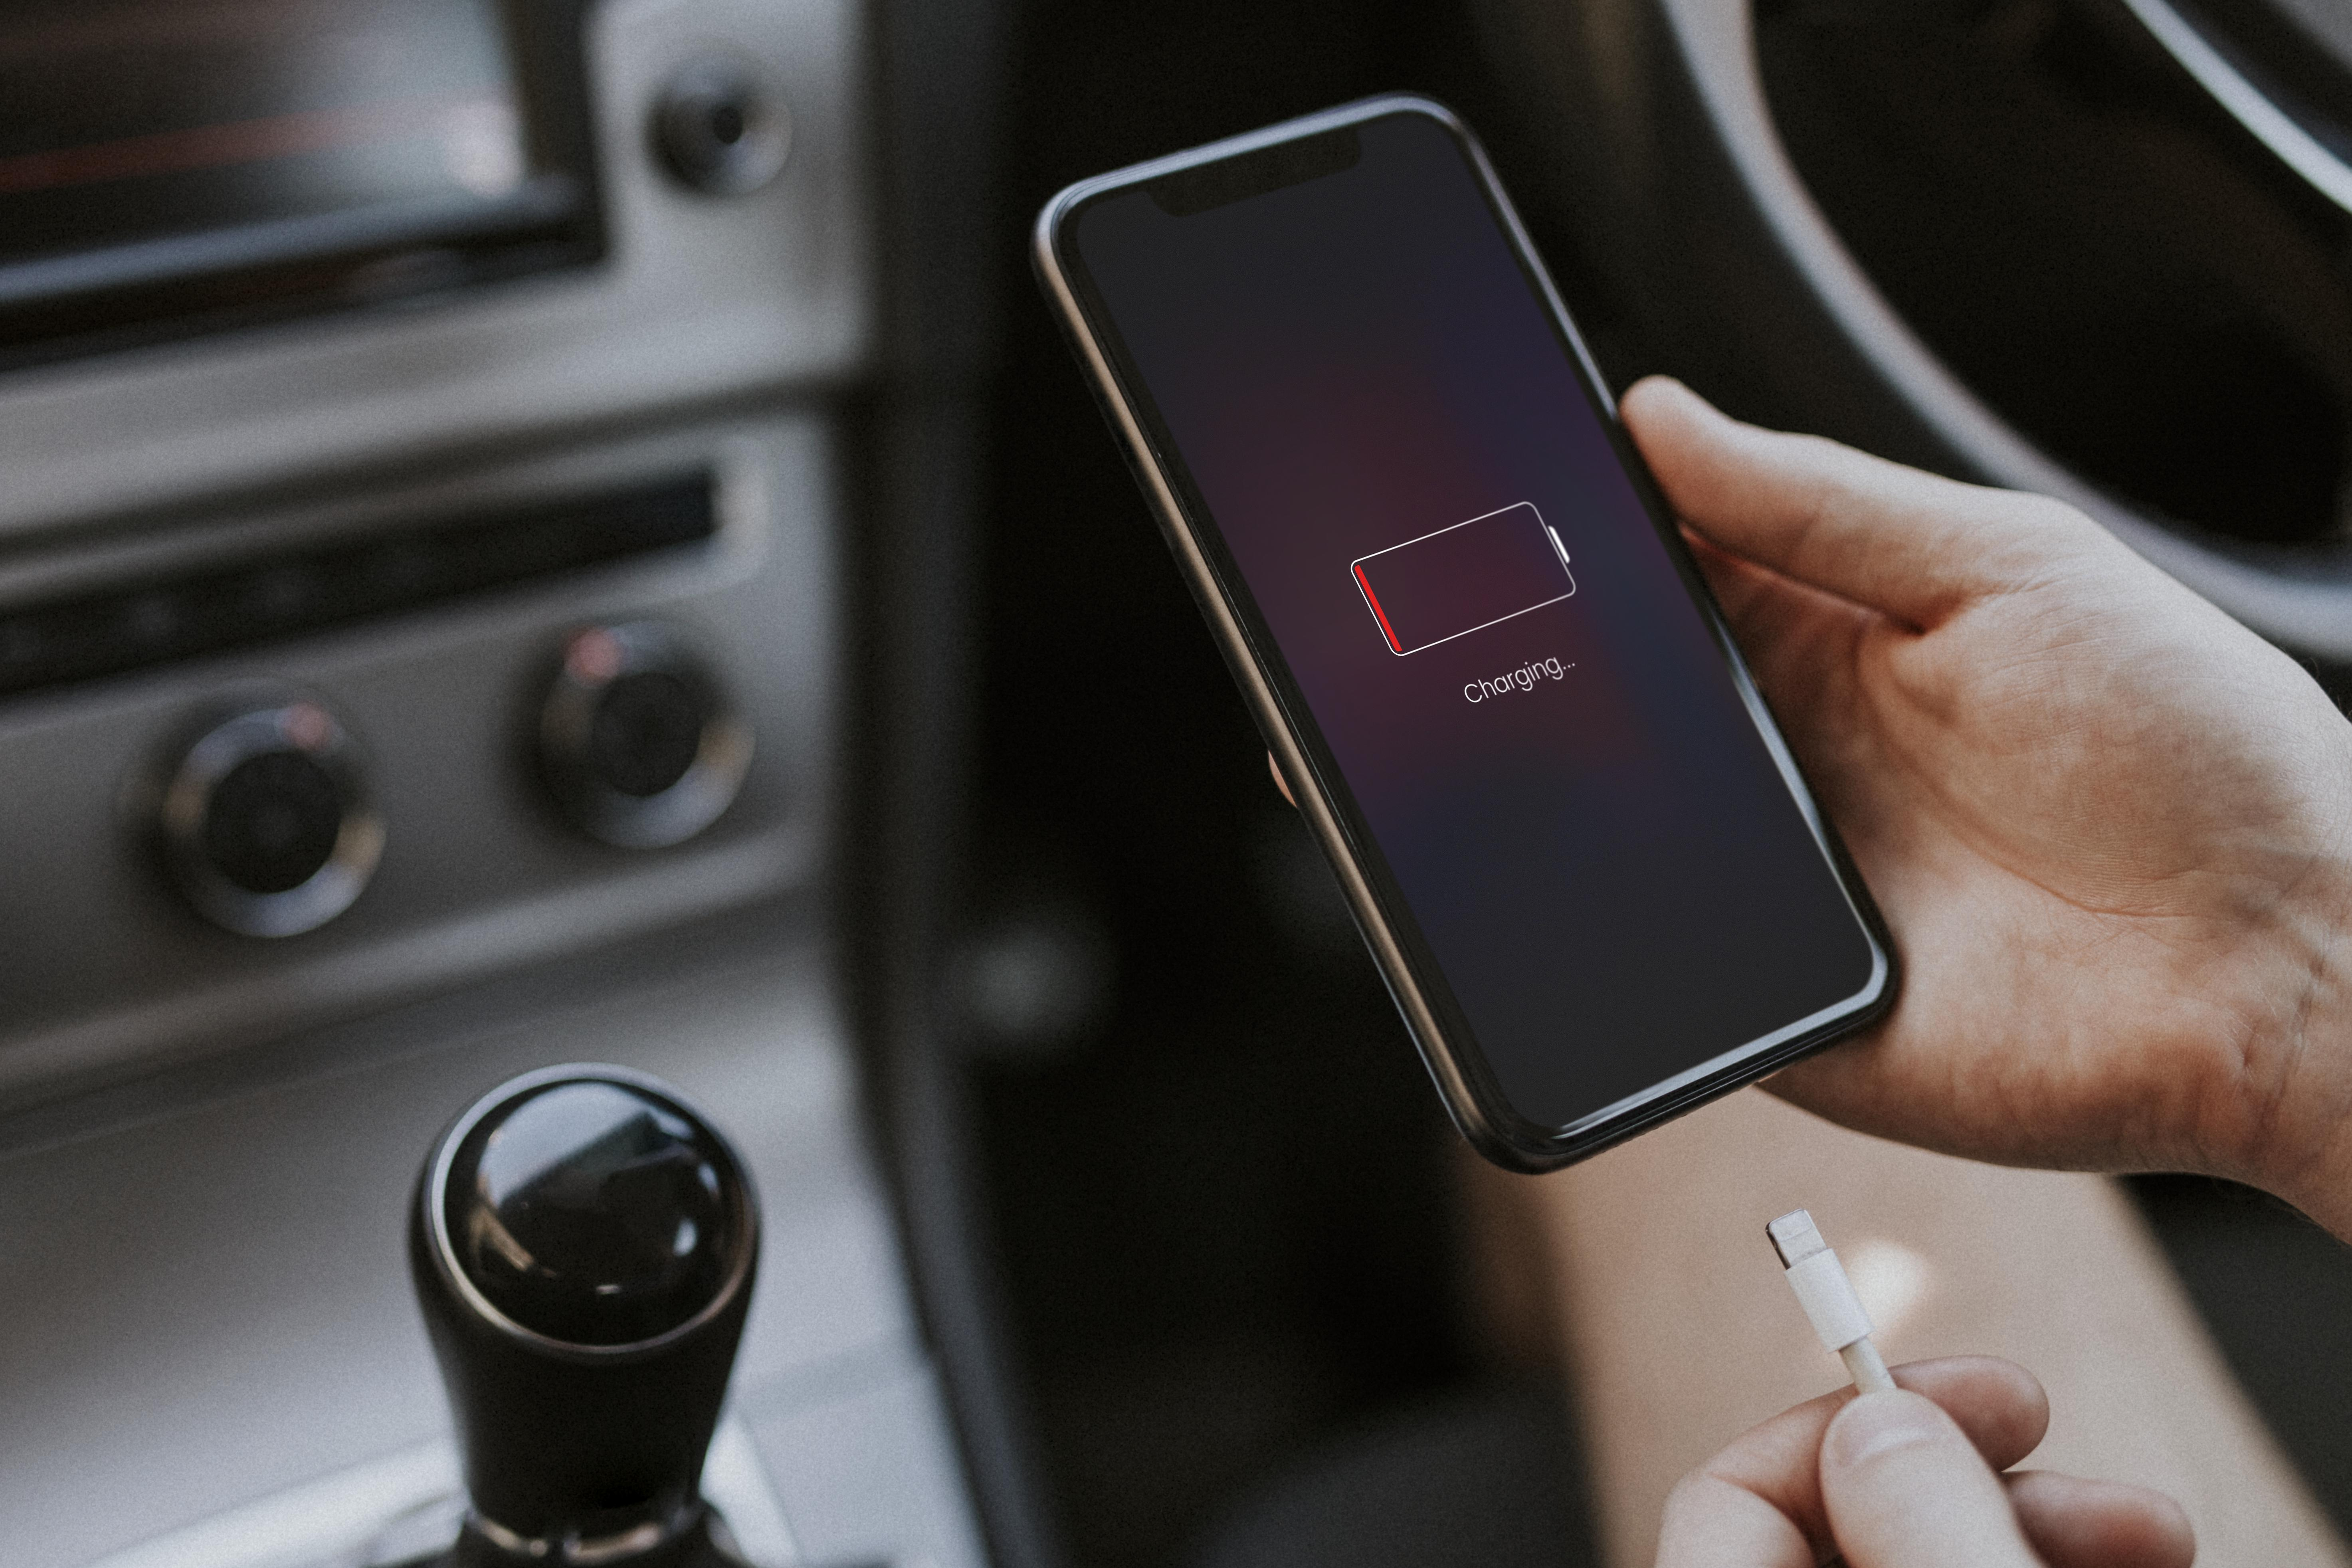
\includegraphics[width=0.8\textwidth]{figures/image.jpeg}
\end{center}

\subsection{Problem Restatement}
\label{subsec:problem}

\hspace*{\parindent}Based on the background discussed above, our goal is to develop a continuous-time mathematical model for a smartphone lithium-ion battery that predicts the State of Charge (SOC) as a function of time and the time-to-empty under various usage conditions. The model should address the following tasks:

\begin{itemize}
    \item \textbf{Develop a Continuous-Time SOC Model:} Grounded in fundamental battery mechanisms, construct a dynamic SOC equation that incorporates multi-factor influences---including screen usage, processor load, and network activity---and perform parameter estimation and validation using publicly available data.

    \item \textbf{Predict Time-to-Empty and Analyze Drivers:} Compute the time-to-empty across representative scenarios, compare predictions against observed behaviors, and identify the key drivers responsible for rapid battery drain.

    \item \textbf{Examine Model Sensitivity:} Analyze how prediction outcomes change with modeling assumptions, parameter values, and fluctuations in usage patterns.

    \item \textbf{Provide Recommendations and Generalization:} Formulate practical guidelines for extending battery life based on model insights, and discuss potential applications in power-saving strategy design and generalization to other portable devices.
\end{itemize}

\subsection{Our Work}
\label{subsec:our-work}

\hspace*{\parindent}We adopt a \textbf{task-driven, multi-model framework} that systematically addresses each problem requirement. The overall workflow of our approach is illustrated in Figure~\ref{fig:workflow}.

\begin{figure}[H]
    \centering
    \begin{tikzpicture}[
        node distance=0.6cm and 0.8cm,
        startstop/.style={rectangle, rounded corners, minimum width=2.2cm, minimum height=0.6cm, text centered, draw=black, fill=green!20, font=\footnotesize},
        process/.style={rectangle, minimum width=2.4cm, minimum height=0.6cm, text centered, draw=black, fill=blue!15, font=\footnotesize},
        model/.style={rectangle, minimum width=2.4cm, minimum height=0.6cm, text centered, draw=black, fill=orange!20, font=\footnotesize},
        output/.style={rectangle, minimum width=2.2cm, minimum height=0.6cm, text centered, draw=black, fill=red!15, font=\footnotesize},
        arrow/.style={thick,->,>=stealth}
    ]
    
    % Row 1: Problem Analysis
    \node (start) [startstop] {Problem Analysis};
    \node (task1) [process, right=of start] {Task 1: SOC Model};
    \node (task2) [process, right=of task1] {Task 2: Prediction};
    \node (task3) [process, right=of task2] {Task 3: Sensitivity};
    \node (task4) [process, right=of task3] {Task 4: Recommend};
    
    % Row 2: Data & Assumptions
    \node (data) [startstop, below=of start] {Data Collection};
    \node (assume) [process, right=of data] {Assumptions};
    
    % Row 3: Model Development
    \node (ecm) [model, below=of data] {2-RC ECM};
    \node (power) [model, right=of ecm] {Power Model};
    \node (thermal) [model, right=of power] {Thermal Model};
    \node (aging) [model, right=of thermal] {Aging Model};
    \node (ode) [model, right=of aging] {5-State ODE};
    
    % Row 4: Analysis & Output
    \node (tte) [output, below=of ecm] {Time-to-Empty};
    \node (monte) [output, right=of tte] {Monte Carlo};
    \node (sobol) [output, right=of monte] {Sobol Analysis};
    \node (valid) [output, right=of sobol] {Validation};
    \node (rec) [output, right=of valid] {Guidelines};
    
    % Arrows - Row 1
    \draw [arrow] (start) -- (task1);
    \draw [arrow] (task1) -- (task2);
    \draw [arrow] (task2) -- (task3);
    \draw [arrow] (task3) -- (task4);
    
    % Arrows - Vertical connections
    \draw [arrow] (start) -- (data);
    \draw [arrow] (data) -- (assume);
    \draw [arrow] (data) -- (ecm);
    \draw [arrow] (assume) -- (power);
    
    % Arrows - Row 3 connections
    \draw [arrow] (ecm) -- (power);
    \draw [arrow] (power) -- (thermal);
    \draw [arrow] (thermal) -- (aging);
    \draw [arrow] (aging) -- (ode);
    
    % Arrows - Row 4 connections
    \draw [arrow] (ecm) -- (tte);
    \draw [arrow] (ode.south) -- ++(0,-0.3) -| (monte.north);
    \draw [arrow] (tte) -- (monte);
    \draw [arrow] (monte) -- (sobol);
    \draw [arrow] (sobol) -- (valid);
    \draw [arrow] (valid) -- (rec);
    
    \end{tikzpicture}
    \caption{Workflow of our multi-model framework for smartphone battery analysis.}
    \label{fig:workflow}
\end{figure}
